\section{Lahirnya Lingkungan St. Theresia Kanak-kanak Yesus}
Pada akhir tahun 2013 yaitu pada bulan September, semua lingkungan di Stasi Maguwo 
diharapkan melakukan pemilihan pengurus baru. Sesuai dengan mekanisme pemilihan dari paroki, 
maka dilakukanlah pemilihan pengurus baru yang diketuai oleh Andreas Keso Muda.
Pemilihan berhasil memilih Anton Supriyana sebagai ketua baru. Beliau ini adalah warga baru namun stok lama. Beliau sudah lama berkecimpung di dewan paroki Pringwulung, tempat tinggal beliau sebelumnya.

\begin{floatingfigure}[l]{2cm}
	\begin{center}
		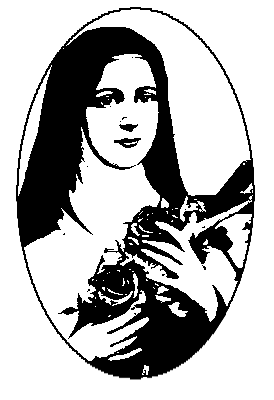
\includegraphics[scale=1]{theresia-logo.png}
	\end{center}
\end{floatingfigure}
Namun karena lingkungan Petrus dirasa terlalu banyak anggotanya, maka atas prakarsa beberapa umat, lingkungan ini diusulkan mekar menjadi 3 dan disetujui oleh umat maupun Dewan Stasi. 

Lingkungan St. Petrus kemudian mekar menjadi Lingkungan Petrus meliputi Kembang, Nanggulan, dan Tobong; Lingkungan St. Monica meliputi Maguwo, Sanggrahan, dan Karangnongko; Lingkungan St. Theresia meliputi Pugeran dan Sombomerten. 


\vspace{0.5cm}


\section{Umat St. Theresia}
Lingkungan St. Theresia mencakup 26 keluarga dengan 82 umat dengan perincian 35 laki-laki dan 47 perempuan. Namun demikian ada beberapa mahasiswa yang terlibat aktif dalam kegiatan-kegiatan lingkungan dan tidak tercatat dengan pasti karena mobilitasnya yang tinggi.

\section{Inventaris Peralatan Misa}
Sejak awal lahirnya lingkungan St. Theresia, umat sudah berkomitmen agar lingkungan mempunyai peralatan misa. Beberapa upaya yang dilakukan adalah pengumpulan data melalui tabungan receh, sumbangan sukarela, dan juga donatur dari luar. Puji syukur kepada Allah bahwa usaha-usaha tersebut banyak membuahkan hasil. Donatur dari luar, berkat ketekunan dari Bapak KRA YP Sunaryo Prononagoro mendapat banyak peralatan misa. 

Peralatan misa yang dimiliki lingkungan antara lain:
\begin{itemize}
\item peralatan altar: salib kuningan dan kayu,
korporal,
purivicatorium,
taplak,
piala,
sibori,
piksis,
patena,
aspergil,
wirug,
krincingan,
tempat lilin besar \& kecil,
patung Bunda Maria,
nampan, ampul,
tempat minyak suci.
\item pakaian liturgi: kasula,
stola,
superpli,
gaun,
kerah lebar,
singel,
alba,
samir
\item buku: buku tpe,
buku liturgi orang sakit,
mazmur tanggapan, sakramen pemberkatan,
aneka ibadat kristiani, teks doa rosario,
puji syukur, teks doa rosario bahasa Jawa.
\item elektronik: ht, \textit{wireless microphone \& speaker}, LCD projector.
\end{itemize} 

Perlu diketahui bahwa patung Bunda Maria Lourdes yang besar adalah sumbangan dari Bapak KRA YP Sunaryo Prononagoro.


